\documentclass{article}
\usepackage[utf8]{inputenc}
\usepackage[english,russian]{babel}
\usepackage{amsmath}
\usepackage[argument]{graphicx}
\usepackage{xcolor}
\usepackage{hyperref}
\usepackage{indentfirst}
\usepackage{algorithm}
\usepackage[noend]{algpseudocode}
\usepackage{caption}

\graphicspath{{charts/}}
\DeclareGraphicsExtensions{.jpg}


\definecolor{linkcolor}{HTML}{799B03} % цвет ссылок
\definecolor{urlcolor}{HTML}{799B03} % цвет гиперссылок
\setlength{\parskip}{0.25cm}
\usepackage[left=2cm,right=2cm,
    top=2cm,bottom=2cm,bindingoffset=0cm]{geometry}

\hypersetup{pdfstartview=FitH,  linkcolor=linkcolor,urlcolor=urlcolor, colorlinks=true}


\title{Преобразование базиса Грёбнера нульмерного идеала к иному мономиальноальному упорядочению.}
\author{Федоров Глеб M33351}
\date{Октябрь 2020}

\begin{document}
\algblock[ALGORITHMBLOCK]{Input}{EndInput}
\algblock[ALGORITHMBLOCK]{Output}{EndOutput}
\algblock[ALGORITHMBLOCK]{Subfunctions}{EndSubfunctions}
\algblock[ALGORITHMBLOCK]{LocalVariables}{EndLocalVariables}

\begin{titlepage}
        \maketitle
\end{titlepage}
    
\section{Оглавление}
    \subsection{Постановка проблемы}
    \subsection{Дополнительная теория}
    \subsection{Алгоритм FGLM}
    \subsection{Примерная архитектура программы}
    \subsection{Используемая литература}
    \newpage
\section{Постановка проблемы}
    Дан базис Грёбнера нульмерного идеала, построенный на мономиальном упорядочении $m_1$.
    Привести данный базис к иному мономиальному упорядочению $m_2$.
    \newpage
\section{Дополнительная теория} 
    \subsection{Исключающий идеал}

    \textbf{Определение:} Пусть дан $I = \langle f_1, \ldots, f_n \rangle  \in F[x_1,\ldots,x_n]$. Тогда l-м исключающим идеалом $I_l$ называется 
    идеал в $F[x_{l+1},\ldots, x_n]$, равный $I \cap F[x_{l+1},\ldots, x_n]$.

    \textbf{Теорема(об исключении):} Пусть $I \subset F[x_1, x_2,\ldots, x_s]$ - идеал и G - его базис Грёбнера по отношению
    к lex-упорядочению с $x_1 > x_2 > \ldots > x_n$. Тогда $\forall l : 0 \leq l \leq n $ множество
    $$G_l = G \cap F[x_1, x_2,\ldots,x_s]$$ является базисом Грёбнера $l$-го исключающего идеала $I_l$.
    
    \textbf{Доказательство:} 
     Зафиксируем $l$ в интервале $(0, n)$. Так как $G_l \in I_l$ по построению, достаточно показать, что 
     $$\langle LT(I_l) \rangle =\langle LT(G_l) f\rangle $$ 
     Включение в одну сторону очевидно
     ($\langle LT(G_l) \rangle \subset \langle LT(I_l) \rangle $ по построению). Докажем, что $\langle LT(I_l) \rangle \subset \langle LT(G_l) \rangle $.
     Для этого достаточно показать что $LT(f)$, где $f \in I_l$, делится на некоторый $g \in G_l$. 
     Заметим, что $f \in I$, то есть $LT(f)$ делится на $LT(g)$ для некоторго $g$(т.к. $G$ является базисом Грёбнера иделала $I$). 
     Так как $f \in I_l$, то $LT(g)$ содержит только переменные $x_{l+1}, \ldots, x_n$. Так как используется lex-упорядочении с 
     $x_1 > x_2 > \ldots > x_n$, то любой моном, содержащий хотя бы одну из переменных $x_1, \ldots, x_l$, больше всех мономов из
     $F[x_{x+1},\ldots, x_n]$. Значит $g\in G_l$, что и требовалось доказать.
    \newpage

    \subsection{Соответсвие иделала и многообразия}

    \textbf{Определение:} Пусть $I \in F[x_1,\ldots, x_n]$ - некоторый идеал. Положим
    $$V(I) = {(a_1, \ldots, a_n) \in F^n : f(a_1, \ldots, a_n) = 0 \:\forall f \in I}$$

    \textbf{Теорема:} $V(I)$ является аффинным многообразием. В частности, если $I = \langle f_1, \ldots, f_n \rangle $, то $V(I) = V(f_1,\ldots,f_n)$

    \textbf{Доказательство:} По теореме Гильберта о базисе идеал $I$ конечно порождён, $I = \langle f_1, \ldots, f_n \rangle $. Покажем, что $V(I) = V(f_1,\ldots,f_n)$.
    Если $f(a_1,\ldots,a_n) = 0$ для всех полиномов $f \in I$, то $f_i(a_1,\ldots,a_n)=0$ (так как $f_i \in I$). Следовательно,
    $V(I) \in V(f_1,\ldots,f_n)$. С другой стороны, пусть $(a_1,\ldots,a_n) \in V(f_1,\ldots, f_n)$, и пусть $f\in I$.
    Так как $I = \langle f_1,\ldots, f_n \rangle $, то $$f = \sum_{i=1}^s h_if_i$$ для некоторых $h_i \in F[x_1, \ldots, x_n]$.
    Но тогда 
    $$f(a_1,\ldots,a_n)=\sum_{i=1}^s h_i(a_1,\ldots,a_n)f_i(a_1,\ldots,a_n)=\sum_{i=1}^s h_i(a_1,\ldots,a_n)*0 = 0$$
    Следовательно, $V(f_1, \ldots, f_n) \in V(I)$, а значит эти два идеала равны. 

    \newpage
    \subsection{Нульмерный идеал}
    \textbf{Определение:} Пусть $A$  - это алгебра над полем $K$ и $J$ - двусторонний идеал в $A$. Рассматривая
    алгебру $A$ как факторкольцо $A/J$, которое можно превратить в алгебру над $K$, если определить в ней умножение
    на элементы поля $K$ следующим образом:
    $$k(a+J) = ka+J, \: \forall k \in K,\: \forall a \in A$$
    Построенная таким образом алгебра называется факторалгеброй алгебры $A$ по идеалу $J$.

    \textbf{Теорема:} Пусть поле $F$ алгебраически замкнуто и $I\in F[x_1, x_2,\ldots, x_n]$.
       Тогда следующие условия эквивалентны:
        
        \begin{enumerate}
            \item Алгебра $A=F[x_1, x_2,\ldots, x_n]/I$ конечномерна над F.
            \item $V(I) \subset F^n$ конечно.
            \item Если $G$ - базис Грёбнера идеала $I$, то $$\forall i \: \exists m_i \geq 0 : x_i^{m_i} = LM(g)$$ для некоторого $g \in G$.
            \item Для каждой переменной $x_i$ исключающий идеал $I \cap F[x_1, x_2,\ldots, x_n]$ является ненулевым.
        \end{enumerate}

      Идеал, удовлетворяюзий данной теореме называется нульмерным

    \newpage

    \subsection{Нормальная форма полинома}

    
    \textbf{Определение(1.1):} Пусть $G$ - базис Грёбнера иделал $I$.
    Будем называть $f \in F[x_1,\ldots,x_n]$ редуцированым по отношению к $G$ (или в нормальной форме по отношению к G), если 
    не существует такого $g \in G$ что его старший член делит какие-либо члены из $f$.
    
    \textbf{Определение:} Алгоритм редукции - алгоритм, вычисляющий нормальную форму полинома $f$.
    
    \textbf{Определение:} Базис Грёбнера $G$ называется редуцированным, если $\forall g \in G$ g - редуцирован по отношению к другим элементам G.
               
    \textbf{Утверждение:} Данное определение редуцированого базиса Грёбнера совпадает с 
    определением из лекции с точностью до нормировки старшего члена.  
     
    \textbf{Определение:} Пусть $I$ - нульмерный идеал над $F[x_1,\ldots,x_n]$ и $G$ - его редуцированный базис Грёбнера.
    Натуральным базисом, определяемым G K-векторного пространства $R/I$, назовем базис $B(G)$, элементами которого являются мономы, редуцированные
    по отношению к $G$. Будем обозначать $D(I)$ размерность $K$-векторного пространства $R/I$(степень идеала).

    \textbf{Определение:} Пусть $B(G)$ - натуральный базис для $R/I$. Тогда положим, что
    $$M(G) = \{x_ib | b \in B(G),\: 1\leq i \leq n,\: x_ib \notin B(G)\}$$ граница $G$.

    \textbf{Теорема(2.1):} Пусть $I$ - нульмерный идеал и $G$ - редуцированный базис Грёбнера данного идеала, и
    B(G) - натуральный базис Грёбнера для $R/I$, тогда $\forall m \in M(G)$ выполнено одно из данных условий:

    \begin{enumerate}
        \item $\forall x_i : x_i | m$ выполнено, что $m/x_i \in B(G)$, тогда и только тогда, когда $m$ - это старший моном элементов из $G$.
        \item $m = x_jm_k$ для некоторых $j$ и $m_k \in M(G)$.
    \end{enumerate}

    \textbf{Доказательство:}
    \begin{enumerate}
        \item Следует из определения редуцированного базиса Грёбнера и определения B(G)
        \item Пусть $x_j$ делит $m$ и $m/x_j \notin B(G)$, тогда $m_k = m/x_j \in M(G)$. Заметим, по определению $M(G)$, что
        $m=x_jm_k=x_ib$. Тогда $i \not= j$(если $i=j$, то $m_k=b$, что противоречит тому, что $m_k \in M(G)$ и $m_k/x_i=b/x_j\in B(G)$, так как $B(G)$, по определению, замкнуто относително деления.
        Таким образом $m_k=x_i(b/x_j)\in M(G)$.
    \end{enumerate}

    \textbf{Следствие:} Пусть $k$ число образующих редуцированного базиса Грёбнера для нульмерного идеала.
        Тогда $k \leq nD(I)$
    
    \newpage    

\section{Алгоритм FGLM}

    \subsection{Вычисление нормальной формы}
    Воспользуемся структурой векторного простраства, чтобы построить алгоритм, который найдёт координаты нормальных форм 
    элементов $R/I$ за полиномиальное время. Для этого рассмотрим n-линейные отображения $\phi_i$  опредлённые на B(G) следующим образом:
    $$\phi_i:\:m\rightarrow NormalForm(x_im)$$.

    \textbf{Определение:}  Обозначим $T(G) = (t_{ijk})$ матрицу $n \times D(I) \times D(I)$, в которой
            $t_{ijk}=j$-ая координата относительно $B(G)$ редукции элементов из $G$ $x_ib_k (b_k \in B(G))$.
 
    Данная матрица будет использована для вычисления нормальной формы полинома.
    
    \textbf{Теорема:} $T(G)$ вычисляется за $O(nD(I)^3)$

    \textbf{Доказательство:} Рассмотрим $MB(G) = B(G) \cup M(G)$ и упорядочим его элементы согласно $m_1$. Будем строить столбцы
    $t_{i*k}$ в том порядке, в котором $x_ib_k$ появляется в $MB(G)$. Рассмотрим $m=x_ib_k$. Если $m \in B(G)$, значит,что $m$ - не 
    редуцирован по отношению к $G$ и другие $t_{ijk} = 0$ для $j \neq k$, и $t_{ikk}=1$. В ином случае $m \in B(G)$, тогда, согласно теореме(2.1), 
    либо $\exists g \in G:\: g=m+\sum_{u=1}^{D(I)} a_ub_u$, тогда $t_{i*k}=(-a_1,\ldots, -a_{D(I)})^t$, либо
    $m=x_lm'$, где $m'\in M(G)$ и $m' < m$. Во втором случае, координаты $m'=x_sb_h$ по отношению к B(G), уже вычислены, и хранятся в $t_{i*k}$. 
    Этого достаточно, чтобы добавить координаты $x_lb_v \: b_v \in B(G)$ умноженые на соответсвующий коэфициент, то есть
    $x_ib_k = x_lx_sb_h = x_l\sum_{v} {t_{svh}b_v}=\sum_u\sum_v{t_{svh}t_{luv}b_u}$. В этом случае мы должны выполнить $D(I)^2$ операций
    чтобы посчитать $t_{i*k}$, и, в итоге, данную операцию мы будем повторять $nD(I)$ раз.

    \textbf{Замечание:} Функция \textit{NextMonom} возвращает следующий моном, который необходимо рассмотреть. О том, как эта функция
    работает будет сказано позднее, но пока будем считать что она выполняется за $O(1)$. 

    \textbf{Замечание:} Для $i \in \{1,\ldots, n\}$ матрица, связанная с $\phi$ относительно $B(G)$, есть $t_{i**}$.
 
    \newpage 
    Данный алгоритм вычисляет конструкцию, описанную на предыдущей странице.

        \begin{algorithm}
        \caption{Matphi}\label{alg:Reduce}
        \begin{algorithmic}[1]
            \Input 
                \State $m_1$
                \Comment{мономиальное упорядочение} 
                \State Basis
                \Comment{минимальный редуцированный базис Грёбнера нульмерного идеала}
            \EndInput
            \Statex 
            \Output
                \State $\phi[i, m, m']$ for $i = 1,\ldots, n$
                \Comment{$m, m'\in B(G)$ такие, что $\phi[i, *, *]$ - это матрица применений $p\rightarrow NormalForm(x_ip)$, где p - редуцированные многочлены} 
            \EndOutput  
            \Statex 
            \Subfunctions
                \State NextMonom
                \Comment{Вовзращает и удаляет первый элемент списка ListOfNexts. Возвращает nil, если список пуст.}
                \State InsertNexts(monom)
                \Comment{Добавляет monom в ListOfNexts и сортирует его, согласно $m_1$}
            \EndSubfunctions
            \Statex 
            \LocalVariables
                \State ListOfNexts
                \Comment{Список "следующих" мономов. Отсортирован относительно $m_1$}
            \EndLocalVariables
            \Statex

            \State $monom := 1$, $ListOfNexts := []$
            \While{$monom \neq null$}
                \If{monom является произведением старших мономов каких-то элементов из Basis}
                    \State{let $monom = x_jm $, где m - редуцируемо относительно Basis}
                    \State{$NormalForm[monom] := \sum\lambda_i*NormalForm(x_jm_i)$}
                    \ForAll{k, таких что $monom = x_km'$, где $m'$ - нередуцируем относительно Basis}
                        \State $\phi[k, m'', m'] :=$ коэфициент $m''$ в $NormalForm[monom]$
                    \EndFor
                \ElsIf{monom - старший моном какого-то $p\in Basis$}
                    \State $NormalForm[monom]:=-rest(p)$
                    \ForAll{j, таких, что $monom = x_jm$}
                        \State $\phi[j,m',m'']:=$ коэфициент $m'$ в $NormalForm[monom]$
                    \EndFor
                \Else
                    \State $NormalForm[monom] := monom$
                    \State $InsertNexts(monom)$
                    \ForAll{j, таких, что $monom = x_jm$}
                        \State {
                        \begin{equation*}
                            \phi[j, m', m] :=  
                             \begin{cases}
                               1 &\text{if $m'=monom$}\\
                               0 &\text{otherwise}
                             \end{cases}
                            \end{equation*}
                        }
                     \EndFor   
                \EndIf        
                $monom := NextMonom$
            \EndWhile    
        \end{algorithmic}
        \end{algorithm}

    \newpage    
    \textbf{Доказательство корректности:}
        Корректность алгоритма следует из доказательства теоремы(2.1). 
        Данный алгоритм представляет собой рассмотрение случаев, рассмотренных в доказательстве данной теоремы и случая, когда полином
        является элементом $B(G)$.

    \newpage
    \subsection{Смена упорядочения}
    \textbf{Теорема(2.2):} Пусть $I$ - нульмерный идеал и $(G_1, m_1)$ - его редуцированный 
    базис Грёбнера, построенный для мономиального упорядочения $m_1$, $m_2$ - иное мономиальное упорядочение. Тогда можно построить
    базис Грёбнера $(G_2, m_2)$ за $O(nD(I)^3)$.
    
    \textbf{Доказательство:} Из $(G_1, m_1)$ мы можем построить $B(G_1) = \{a_1,\ldots,a_{D(I)}\}$, $M(G_1)$ и $T(G_1)$, как
    было показано в предыдущей главе. Построим матрицу $C$ в которой $i-$й столбец будет координатами элемента $b_i \in B(G_2)$
    относительно $B(G_1)$.
    Будем строить новый базис итеративно.
    Пусть $B(G_2) := \{1\}$ и $M(G_2) := \emptyset$. Пусть $m = min_{m_2} \{x_jb_i | 1\leq j \leq n, b_i \in B(G_2), 
    x_jb_i\notin B(G_2)\cup M(G_2)\}$. Может возникнуть три случая:
    \begin{enumerate}
        \item m - старший терм g, какого-либо $g \in G_2$
        \item m нужно добавить в $B(G_2)$
        \item m нужно добавить в $M(G_2)$, но m - кратно $LT(G)$ для некоторого $g \in G$.
    \end{enumerate}
    Проверка того, что $m$ удовлетворяет третьему пункту - старший член $g$ строго меньше чем $m$ при любом допустимом упорядочении
    и $g$ уже добавлен в $M(G_2)$.
    Поскольку по построению, $m=x_jb_i$ мы можем посчитать его координаты $c(m)_h$ относительно $B(G_1)$ используя матрицы $C$ и $T(G_1) = (t_{ijk})$:
    $$m=x_jb_i=x_j*\sum_k c_{ki}*a_k = \sum_k x_j*c_{ki}*a_k = \sum_k c_{ki}*\sum_h t_{jhk}*a_h = \sum_h (\sum_k t_{jhk}c_{ji}) = \sum_h c(m)_ha_h$$
    Если вектор $c(m)$ линейно независим от векторов из $C$, то выполняется второй пунк, и мы нашли новый $g \in B(G_2)$. В противном случае,
    мы получаем элемент $g \in G_2$.
    \newpage

        \begin{algorithm}
        \caption{NewBasis}\label{alg:Conversion}
        \begin{algorithmic}[1]
            \Input
            \State $m_2$ 
            \Comment{новое упорядочение}
            \State oldBasis 
            \Comment{Базис Грёбнера нульмерного идела относительно упорядочения $m_1$}
            \EndInput

            \Statex 
            \Output
            \State newBasis 
            \Comment{Базис Грёбнера нульмерного идеала относительно упорядочения $m_2$}
            \EndOutput

            \Statex 
            \Subfunctions
            \State NormalForm(polynom) 
            \Comment{Возвращает редуцированную форму полинома относительно oldBasis и $m_1$}
            \State NextMonom() 
            \Comment{Возвращает первый элемент ListOfNexts или nil, если ListOfNexts пуст. Первый элемент удаляется}
            \State InsertNexts(monom)
            \Comment{Добавляет в ListOfNexts произведение монома со всеми переменными, после чего сортирует список относительно $m_2$ и удаляет дубли}
            \EndSubfunctions
            
            \Statex 
            \LocalVariables
            \State staircase 
            \Comment{Список ведущих мономов из NewBasis}
            \State MBasis 
            \Comment{Список пар $[a_i, b_i]$, где $a_i$ - мономы в нормальной форме относительно нового базиса и 
            $b_i = NormalForm(a_i)$, нормальная форма $a_i$ относительно старого базиса.}
            \State ListOfNexts 
            \Comment{Список "следующих" мономов. Отсортирован относительно $m_2$}
            \EndLocalVariables

            \Statex 
                \State {$MBasis := []; staircase := []; newBasis := []; ListOfNexts := []; monom := 1;$}
                \While {$monom \neq nil$}
                    \If {monom не является произведением элементов из staircase}
                    \Comment{Провекра, это пункт 1 или 2}
                        \State $vector := NormalForm(monom)$
                        \Comment{}
                        \If {есть линейная зависимость $vector + \sum_{v \in MBasis} \lambda_v second(v) = 0$}
                            \State $pol := monom + \sum_{v \in MBasis} \lambda_v first(v)$ 
                            \State $newBasis := cons(pol, newBasis)$
                            \State $staircase := cons(monom, staircase)$
                        \Else
                            \State $MBasis := cons([monom, vector], MBasis)$
                            \State InsertNexts(monom)
                        \EndIf
                    \EndIf
                    \State monom := NextMonom
                \EndWhile
            
        \end{algorithmic}
        \end{algorithm}
  
    \newpage
    \textbf{Доказательство корректности:}

        \textbf{Первое:} Покажем, что \textit{newBasis} - это базис Грёбнера того же идеала при упорядочении $m_2$. 
        Для этого покажем, что элементы из \textit{MBasis} независимы по модулю идеала, порождаемого \textit{oldBasis}. Пусть это не так
        тогда существует линейная комбинация элементов из $MBasis$ $P = \sum \lambda_i*m_i$, такая, что $P\in \langle oldBasis\rangle$. Тогда
        $$NormalForm(P) = \sum \lambda_i NormalForm(m_i) = 0$$
        ...

        \textbf{Второе:} Покажем что алгоритм завершается. 
        Заметим, что дан нульмерный идеал. Это значит, что максимальное число линейно независимых нередуцируемых конечно, и равно
        отношению размерноси кольца многочленов к размерносит идеала, то есть числу нередуцируемых одночленов для любого базиса Грёбнера.
        Таким образом, число итераций, которые увеличивают \textit{MBasis} конечно. После того, кок все элементы \textit{MBasis} рассмотрены,
        \textit{ListOfNexts} не будет больше увеличиваться, значит, количество оставшихся итераций конечно.
    \newpage
    \textbf{Реализация \textit{NextMonom}:}
        При вставке одночлена в $ListOfNexts$ полезно помнить, что он получается как произведение переменной на одночлен с известной нормальной формой.
        При этом один и тот же моном можно получить несколько раз... 
    \newpage
\section{Примерная архитектура программы}

\begin{figure}[h!]
    \center{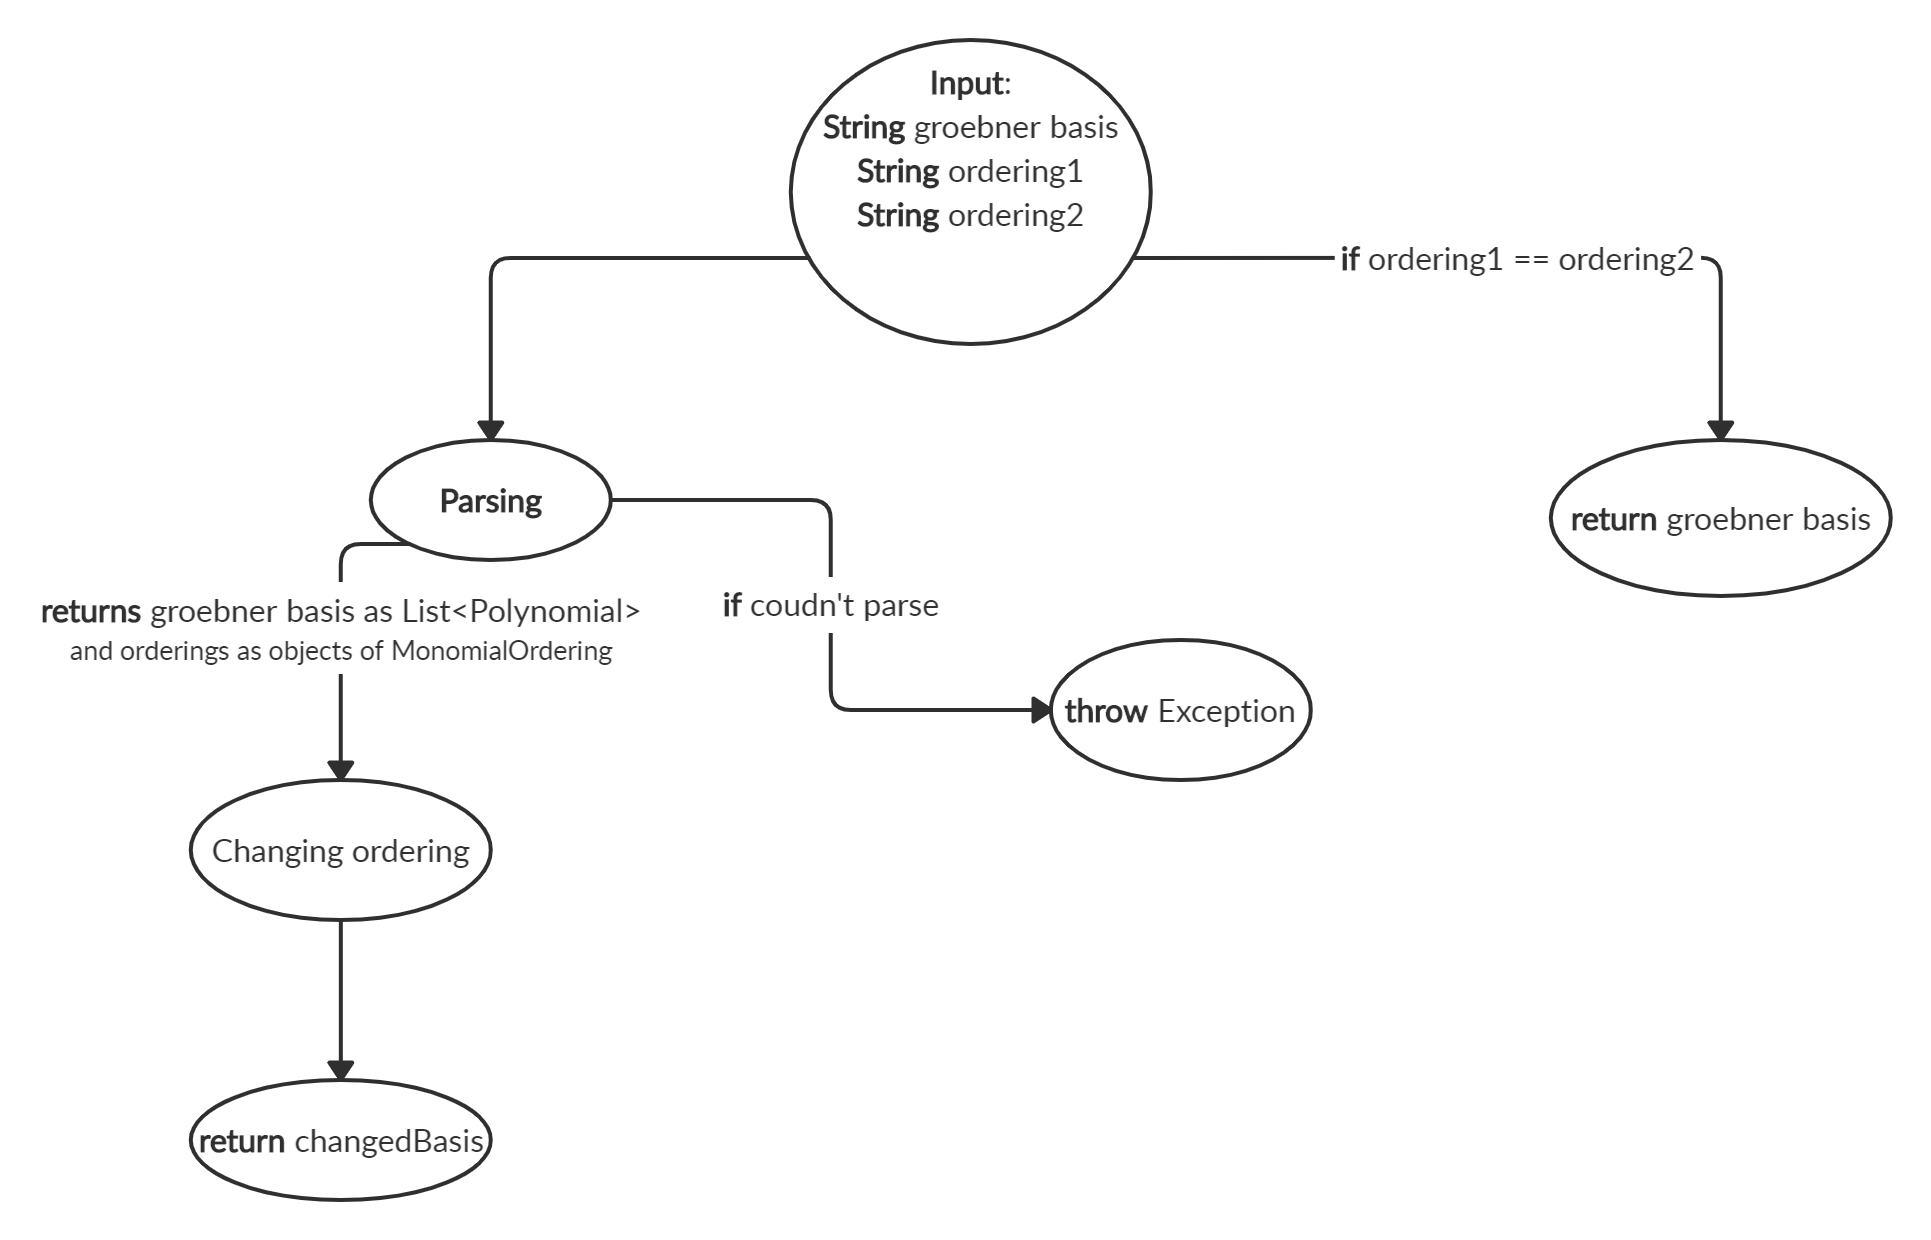
\includegraphics[scale=0.25]{General scheme}}
    \caption{Схема работы программы}
\end{figure}
\newpage
\section{Используемая литература}
\begin{enumerate}
    \item Faugère, J.C., Gianni, P., Lazard, D., Mora, T. Efficient computation of zero-dimensional gröbner bases by change of ordering (1993) Journal of Symbolic Computation, 16 (4), pp. 329-344.
    \item \href{http://halgebra.math.msu.su/groebner.pdf}{http://halgebra.math.msu.su/groebner.pdf}
    \item Кокс Д., Литтл Дж., О'Ши Д. Идеалы, многообразия, кольца. Стр. 108. Стр. 153. 
    \item \href{https://www.math.lsu.edu/system/files/Groeb_presentation_final.pdf}{Презентация про FGLM алгоритм}
\end{enumerate}

\end{document}